 \documentclass[12pt,a4paper]{article}

\usepackage{graphicx}% Include figure files
\usepackage{dcolumn}% Align table columns on decimal point
\usepackage{bm}% bold math
%\usepackage{hyperref}% add hypertext capabilities
%\usepackage[mathlines]{lineno}% Enable numbering of text and display math
%\linenumbers\relax % Commence numbering lines

%\usepackage[showframe,%Uncomment any one of the following lines to test 
%%scale=0.7, marginratio={1:1, 2:3}, ignoreall,% default settings
%%text={7in,10in},centering,
%%margin=1.5in,
%%total={6.5in,8.75in}, top=1.2in, left=0.9in, includefoot,
%%height=10in,a5paper,hmargin={3cm,0.8in},
%]{geometry}

\usepackage{multicol}%Para hacer varias columnas
\usepackage{multicol,caption}
\usepackage{multirow}
\usepackage{cancel}
\usepackage{hyperref}
\hypersetup{
    colorlinks=true,
    linkcolor=blue,
    filecolor=magenta,      
    urlcolor=cyan,
}

\setlength{\topmargin}{-1.0in}
\setlength{\oddsidemargin}{-0.3pc}
\setlength{\evensidemargin}{-0.3pc}
\setlength{\textwidth}{6.75in}
\setlength{\textheight}{9.5in}
\setlength{\parskip}{0.5pc}

\usepackage[utf8]{inputenc}
\usepackage{expl3,xparse,xcoffins,titling,kantlipsum}
\usepackage{graphicx}
\usepackage{xcolor} 
\usepackage{siunitx}
\usepackage{nopageno}
\usepackage{lettrine}
\usepackage{caption}
\renewcommand{\figurename}{Figura}
\usepackage{float}
\renewcommand\refname{Bibliograf\'ia}
\usepackage{amssymb}
\usepackage{amsmath}
\usepackage[rightcaption]{sidecap}
\usepackage[spanish]{babel}

\providecommand{\abs}[1]{\lvert#1\rvert}
\providecommand{\norm}[1]{\lVert#1\rVert}
\newcommand{\dbar}{\mathchar'26\mkern-12mu d}

\usepackage{mathtools}
\DeclarePairedDelimiter\bra{\langle}{\rvert}
\DeclarePairedDelimiter\ket{\lvert}{\rangle}
\DeclarePairedDelimiterX\braket[2]{\langle}{\rangle}{#1 \delimsize\vert #2}

% CABECERA Y PIE DE PÁGINA %%%%%
\usepackage{fancyhdr}
\pagestyle{fancy}
\fancyhf{}

\begin{document}

Macías Márquez Misael Iván

\begin{enumerate}


%%%1%%%



\item Una partícula de masa $m$ se mueve sin fricción sobre una superficie cónica bajo la acción de la gravedad. El ángulo entre el eje del cono y la generatriz es $\alpha$.

    \begin{figure}[h!]
        \centering
        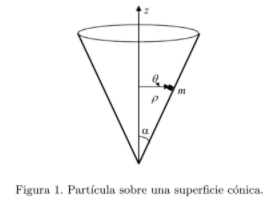
\includegraphics{1.PNG}
    \end{figure}

\begin{enumerate}
    \item Determine el lagrangiano de la partícula en términos solamente de las coordenadas cilíndricas $\rho$ y $\theta$.
    
    \textbf{Sol:}
    
    El lagangiano en coordenadas cartesianas para este sistema está descrito por
    
    \begin{equation*}
        L = \frac{1}{2} m (\dot{x}^2 + \dot{y}^2 + \dot{z}^2)  - mgz
    \end{equation*}
    
    entonces como el cono en cilíndricas es de la forma $z = \frac{\rho}{\sin{\alpha}} $ y por la relación de coordenadas $x = \rho \cos{\theta}$  $y = \rho \sin{\theta}$, la lagrangiana queda como
    
    \begin{equation*}
        L = \frac{1}{2} m [(\dot{\rho} \cos{\theta}- \rho \sin{\theta} \dot{\theta})^2 + (\dot{\rho} \sin{\theta}+ \rho \cos{\theta}\dot{\theta})^2 + (\dot{\rho}/\sin{\alpha})^2] - mg\rho/\sin{\alpha}
    \end{equation*}
    
    \begin{equation*}
        = \frac{1}{2}m [\dot{\rho}^2 (\cancel{\cos^2{\theta} + \sin^2{\theta}} + 1/\sin^2{\alpha}) + \rho^2 \dot{\theta}^2 \cancel{(\cos^2{\theta} + \sin^2{\theta})}] - mg\rho / \sin{\alpha}
    \end{equation*}
    
    por lo tanto
    
    \begin{equation*}
        L (\rho,\dot{\rho}, \dot{\theta})= \frac{1}{2}m \left(\frac{\sin^2{\alpha + 1}}{\sin^2{\alpha}} \dot{\rho}^2 + \rho^2 \dot{\theta}^2\right) - \frac{mg \rho}{\sin{\alpha}}
    \end{equation*}
    
    \item ¿Existe alguna variable cíclica? En caso afirmativo, identifique la correspondiente cantidad física que se conserva. Use este hecho para encontrar la ecuación para $\rho$.
    
    \textbf{Sol:}
    
    Dado que la lagrangiana no depende explícitamente de $\theta$, $\theta$ debe ser una variable cíclica y también $\frac{\partial L}{\partial \dot{\theta}} = p_{\theta} = m \rho^2 \dot{\theta}$ es una cantidad conservada por lo que
    
    \begin{equation*}
        \frac{d p_{\theta}}{d t} = \frac{\partial p_{\theta}}{\partial \rho} \dot{\rho} + \frac{\partial p_{\theta}}{\partial \dot{\theta}} \ddot{\theta}= 0
    \end{equation*}
    
    \begin{equation*}
        = 2m\rho \dot{\theta} \dot{\rho} + m \rho^2 \ddot{\theta} = 0
    \end{equation*}
    
    \begin{equation*}
        \frac{\dot{\rho}}{\rho} =(- 1/2) \frac{\ddot{\theta}}{\dot{\theta}}  \hspace{1cm} \rightarrow \hspace{1cm} \rho = \dot{\theta}^{-1/2} + c
    \end{equation*}
    
    \item Muestre que este problema se reduce al movimiento unidimensional de una partícula en un potencial efectivo $V_{ef} (p)$. Haga un esbozo de $V_{ef}(p)$.
    
    \textbf{Sol:}
    
    como $p_{\theta}$ es una cantidad conservada, se cumple que $p_{\theta} = m \rho^2 \dot{\theta} = cte$ por lo que la energía del sistema se puede escribir como
    
    \begin{equation*}
        E = \frac{1}{2}m \dot{r}^2 + \frac{1}{2} \frac{p_{\theta}^2}{m \rho^2} + \frac{mg \rho}{\sin{\alpha}}
    \end{equation*}
    
    con un potencial efectivo $V_{ef} = \frac{1}{2} \frac{p_{\theta}^2}{m \rho^2} + \frac{mg \rho}{\sin{\alpha}}$, y por la conservación de la energía se puede llegar a
    
    \begin{equation*}
        \theta = \int \frac{p_{\theta} d\rho}{\rho^2 \sqrt{2m(E-V) - p_{\theta}^{2}/\rho^2}}+ c
    \end{equation*}
    
    por lo que se reduce a un problema unidimensional
    
    \begin{figure}[h!]
        \centering
        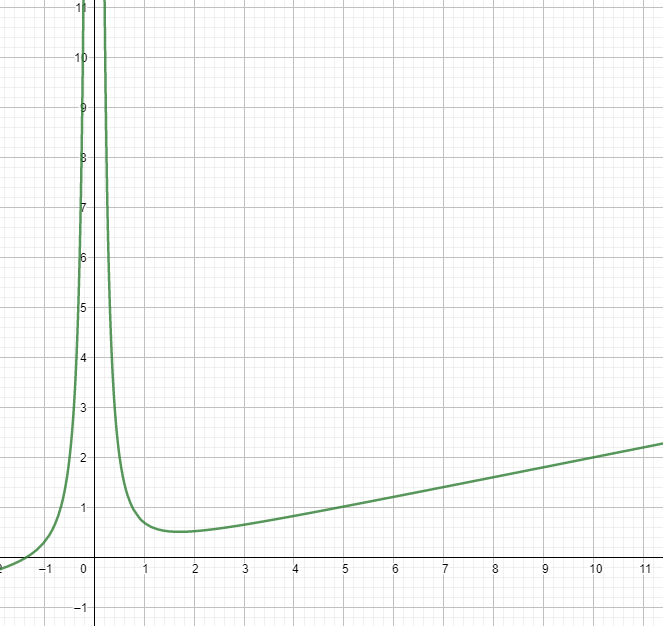
\includegraphics[scale=0.5]{1,c.PNG}
    \end{figure}
    
    
    
    \item Si la partícula es lanzada horizontalmente con la velocidad $\mathbf{v}= v_0 \mathbf{e}_{\theta}$ a la altura $z_0$, muestre que la condición para un movimiento circular es $v_0 ^2 = g z_0$.
    
    \textbf{Sol:}
    

    
    
\end{enumerate}



%%%2%%%



\item Para un potencial atractivo $1/r$ de fuerza central mostrar lo siguiente:

\begin{enumerate}
    \item Dada una órbita circular y una parabólica con el mismo momento angular, la distancia al perihelio de la parábola es la mitad del radio del círculo
    
    \textbf{Sol:}
    
    como vimos, este problema queda descrito con
    
    \begin{equation*}
        r = \frac{p_\phi}{1 + e \cos{\phi}}
    \end{equation*}
    
    entonces la excentricidad es $e = 0$ para el círculo, que sustituyendo nos da $r' = p_{\phi}= mr^2 \dot{\phi}^2$, ahora para la parábola $e = 1 $ por lo que $r = \frac{p_{\phi}}{1 + \cos{\phi}}$, la distancia al perihelio que está en el origen cuando $\phi = 0$ es $r = p_{\phi}/2 = r' /2$
    
    
    
    \item La velocidad de la partícula en cualquier punto sobre la órbita parabólica es $\sqrt{2}$ veces la velocidad de la partícula sobre la órbita circular (sobre el mismo punto).
    
    \textbf{Sol:}
    
    El vector velocidad en coordenadas polares se escribe como $v^2 = \dot{r}^2 + r^2 \dot{\phi}^2 $, entonces para el círculo $\dot{r} = 0$ por lo que  $v^2 = r^2 \dot{\phi}^2 $  o bien $v_c = \sqrt{\frac{p_{\phi}}{m}}$, ahora para la parábola  $\dot{r} = p_{\phi} \frac{\sin{\phi}}{(1 + \cos{\phi})^2} $ y entonces
    
    \begin{equation*}
        v^2 = r^2 \dot{\phi}^2 \left(\frac{\sin^2{\phi}}{(1+\cos{\phi})^2} + 1\right) = r^2 \dot{\phi}^2 \left(\frac{\sin^2{\phi} + (1+\cos{\phi})^2}{(1+\cos{\phi})^2}\right)
    \end{equation*}
    
    \begin{equation*}
        = \frac{2r^2 \dot{\phi}^2}{1+ \cos{\phi}} = \frac{2r^3 \dot{\phi}^2}{p_{\phi}} = 2 \frac{p_{\phi}}{m} \hspace{1cm} \rightarrow \hspace{1cm} v = \sqrt{2} \sqrt{ \frac{p_{\phi}}{m}} = \sqrt{2} v_c
    \end{equation*}
    
    
    
\end{enumerate}



%%%3%%%



\item Una partícula de masa $m$ se mueve en una órbita circular de radio $R$ bajo la influencia de la fuerza atractiva central,

\begin{equation*}
    f(r) = - \frac{k}{r^2} e^{-r/a}
\end{equation*}

donde $k$ y $a$ son constantes positivas.

\begin{enumerate}
    \item Determine la condición que debe cumplir $a$ para el movimiento circular sea estable.
    
    \textbf{Sol:}
    
    
        Supongamos que el radio de la orbita es $r'$, $f = -\frac{d U}{dr}$ entonces $U= -\frac{k}{r}e^{-r/a}$ por lo la lagrangiana del sistema queda como
        
        \begin{equation*}
            L = \frac{1}{2} m (\dot{r}^2 + r^2 \dot{\theta}^2) + \frac{k}{r} e^{-r/a}
        \end{equation*}
        
        de donde obtenemos el potencial efectivo $U_{ef} = \frac{p_{\theta}^2}{2mr^2} - \frac{k}{r} e^{-r/a}$, ahora para tener una orbita circular es necesario tener $\frac{d U_{ef}}{dr} = 0 $ o bien $e^{-r/a} \frac{r}{a}(1 + r/a) = \frac{p_{\theta}^2}{mka}$, y así tenemos que
        
        \begin{equation*}
            U_{min} = \frac{p_{\theta}^2}{2mr'} \frac{a-r'}{a+r'}
        \end{equation*}
        
        por lo tanto $a$ debe ser distinto de $-r'$ y $0$
    
    \item Calcule la frecuencia de las pequeñas oscilaciones radiales respecto al movimiento circular
    
    \textbf{Sol:}
    
    \begin{equation*}
        \omega = \sqrt{\frac{\frac{\partial^2 U}{\partial r^2}}{m}} = \sqrt{\frac{-ke^{-r/a}}{rm} (\frac{2}{r^2} + \frac{2}{ra} + \frac{1}{a^2})}
    \end{equation*}
    
\end{enumerate}



%%%4%%%




\item Un péndulo de masa $m$ está suspendido de un bloque de masa $M$ que puede desplazarse sin fricción a lo largo de una recta horizontal

\begin{figure}[h!]
    \centering
    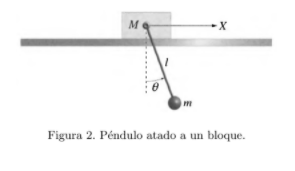
\includegraphics{2.PNG}
\end{figure}

\begin{enumerate}
    \item Determine el lagrangiano de este sistema en términos de las coordenadas $x$ y $\theta$.
    
    \textbf{Sol:}
    
    Las coordenadas del las masas son
    
    \begin{equation*}
        x_M = x \hspace{1cm} y_M = 0
    \end{equation*}
    
    \begin{equation*}
        x_m = x + l \sin{\theta} \hspace{1cm} y_{m} = l \cos{\theta}
    \end{equation*}
    
    por lo que el lagrangiano queda como
    
    \begin{equation*}
        L = K_M + K_m - \cancel{U_M} - U_m
    \end{equation*}
    
    \begin{equation*}
        = \frac{1}{2}M (\dot{x}_{M}^{2} + \cancel{\dot{y}_{M}^2}) + \frac{1}{2} m (\dot{x}_{m}^{2} + \dot{y}_{m}^{2}) + mgy_m
    \end{equation*}
    
    \begin{equation*}
        = \frac{1}{2}M \dot{x}^{2}  + \frac{1}{2} m ((\dot{x} + l \cos{\theta}\dot{\theta})^{2} + (-l\sin{\theta}\dot{\theta})^{2}) + mgl \cos{\theta}
    \end{equation*}
    
    \begin{equation*}
        \therefore L = \frac{1}{2}(m+M) \dot{x}^2 + \frac{1}{2} m (l^2 \dot{\theta}^2 + 2l \dot{x}\dot{\theta}\cos{\theta}) + mgl \cos{\theta}
    \end{equation*}
    
    \item Obtenga el lagrangiano de este sistema en la vecindad de su estado de equilibrio estable.
    
    \textbf{Sol:}
    
    Primero para tener un punto de equilibrio estable, necesitamos un máximo del potencial $U= mgl\cos{\theta}$ el cual se da para  $\theta = 0$ debido a que $\frac{d U}{d \theta} = 0$ para $\theta = 0 , \pi$ y  $\frac{d^2 U}{d \theta^2} > 0$ para $\theta = 0$.
    
    Ahora desarrollando el potencial $U(\theta)$ sobre $0$ y usando la aproximación de pequeñas desviaciones, llegamos a
    
    \begin{equation*}
        L (\theta) = \frac{1}{2} m \dot{\theta}^2 + \frac{1}{2} k \theta =\frac{1}{2} m \dot{\theta}^2 + \frac{1}{2} mgl\cos{\theta} \theta
     \end{equation*}
    
    \item Determine la frecuencia de las oscilaciones pequeñas de este sistema.
    
    \textbf{Sol:}
    
    Ya que $k = \frac{d^2 U}{d \theta ^2}$
    
    \begin{equation*}
        \omega = \sqrt{\frac{k}{m}} = \sqrt{gl\cos{\theta}}
    \end{equation*}
    
\end{enumerate}
    
\end{enumerate}

\end{document}